\documentclass[sigconf]{acmart}
% use \code{foobar} for monospace (instead of \texttt{qux})
\newcommand{\code}{\texttt}

\usepackage{booktabs} % For formal tables
\usepackage{graphicx}
\usepackage[english]{babel}



\begin{document}
\settopmatter{printacmref=false} % Removes citation information below abstract
\renewcommand\footnotetextcopyrightpermission[1]{} % removes footnote with conference information in first column
\pagestyle{plain} % removes running headers

\title{Cryptocurrency Market Prediction Using Twitter}
\subtitle{Milestone 1 Update}

\author{Will Badart}
\affiliation{%
  \institution{University of Notre Dame}
  \city{South Bend}
  \state{Indiana}
}
\email{wbadart@nd.edu}

\author{Matthew Fabian}
\affiliation{%
  \institution{University of Notre Dame}
  \city{South Bend}
  \state{Indiana}
}
\email{mfabian@nd.edu}

\author{Shane Ryan}
\affiliation{%
  \institution{University of Notre Dame}
  \city{South Bend}
  \state{Indiana}
}
\email{sryan8@nd.edu}

\author{Mara Staines}
\affiliation{%
  \institution{University of Notre Dame}
  \city{South Bend}
  \state{Indiana}
}
\email{mstaines@nd.edu}


\begin{abstract}
Cryptocurrency as a commodity has proven to be quite volatile, making prediction of market trends highly valuable. Our team will leverage the constant stream of tweets discussing cryptocurrency on Twitter in order to build a model that can predict changes in a cryptocurrency's value.
\end{abstract}

\maketitle


\section{Introduction}
Every day, Twitter users produce more than 500 million tweets\cite{sayce}. This makes Twitter an ideal resource for social sensing --- the use of humans as sensors. Users tweet and retweet about events, places, emotions, and more; the aggregation of this data has proven powerful for event detection and prediction. One of the fastest-growing conversations taking place on the platform is over cryptocurrency.

Cryptocurrency is a growing market that is both widely discussed and highly volatile, leading our team to believe that tweets may reflect trends in cryptocurrency value. Successfully using Twitter data to predict changes in cryptocurrency markets would provide a significant advantage in cryptocurrency trading. In this project, we will build a model to predict changes in the value of several major cryptocurrencies based on real-time data from Twitter.


\section{Approach}

\subsection{Data Sources}
Data for this project will come from Twitter. We will stream tweets using the Twitter API, which allows for tweets to be collected in near real-time. We will use the filtering capability of the Twitter API to only collect tweets that contain certain keywords. We have selected both general keywords (e.g. \code{cryptocurrency}, \code{altcoin}) and keywords for the specific cryptocurrencies we will be exploring (e.g. \code{bitcoin}, \code{BTC}, \code{ethereum}). If a tweet contains one or more of these keywords, our program will store the tweet body as well as important metadata (user ID, timestamp, retweets, favorites, etc.) in JSON format and append it to a data file.

Many sites provide historical data on cryptocurrency value. We will be utilizing the API of \href{https://www.cryptocompare.com}{CryptoCompare.com} to retrieve cryptocurrency values for the timespan of the tweet data.

\subsection{Methodology}
Once data is collected from Twitter, it will be cleaned, categorized, and used in a regression model to make predictions. Twitter data is noisy, so the first component of data processing will be to eliminate tweets irrelevant to cryptocurrency which made it past the API filter. Our strategy for this task is to use a clustering algorithm to group tweets as relevant or noise. Because tweets are collected based on keywords, features for clustering include measures such as where in the tweet the keyword is located, or what words occur before and after the keyword. This method has been proven effective for removing irrelevant tweets from a set of tweets collected during an event by keyword\cite{sakai}. A similar method (potentially in conjunction with a named entity recognition step) will be used to categorize which cryptocurrencies a tweet is referring to.

Once noise is removed and each tweet is labeled with the currency (or currencies) to which it refers, data from the tweets will be used to calculate features in a regression algorithm predicting market trends for various currencies. Features may include number of tweets and sentiment/ mood of tweets.

First, we hope to take tweets from an entire day as input, and output the predicted change in currency value from one day to the next. After we have a strong model at this level, we will work on increasing granularity over time for our predictions. An ideal model would provide the predicted change in currency value every minute in order to influence trading decisions.


\begin{figure}[H]
\caption{Flow of data processing}
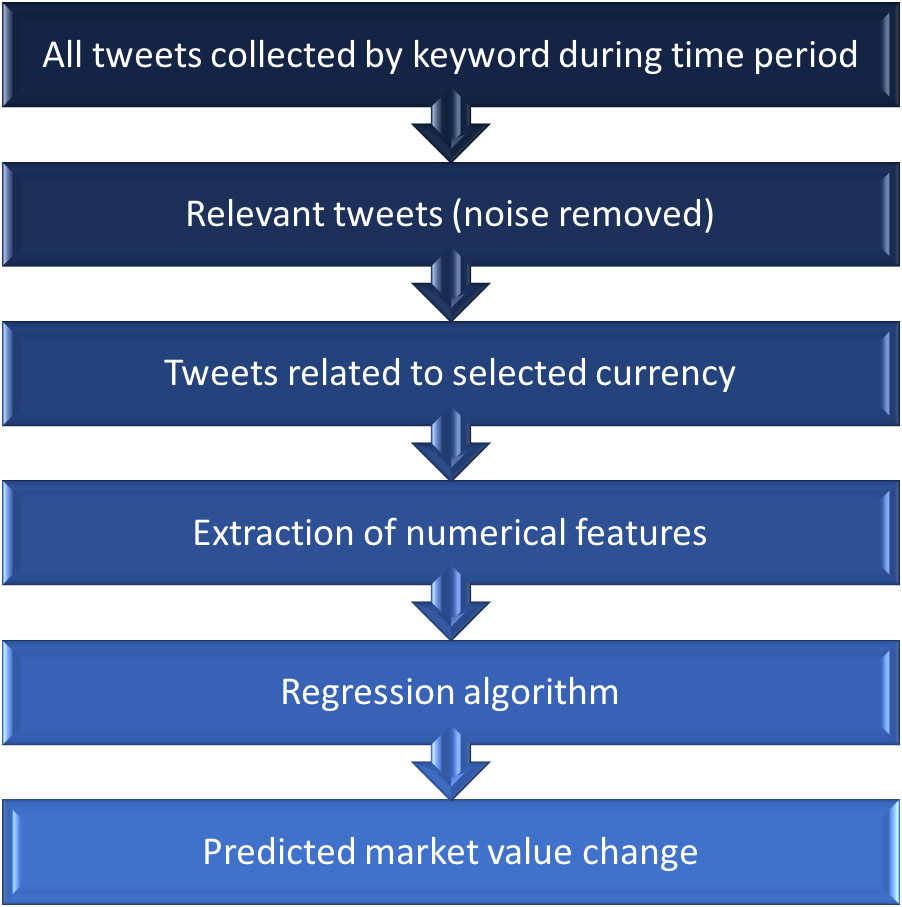
\includegraphics[width=7cm]{chart.png}
\end{figure}


\section{Evaluation Plan}
Evaluation for our model relies on knowledge of actual cryptocurrency values over time, which will be gathered from CryptoCurrency.com. Comparison of our predicted changes to actual changes can be calculated with statistical methods such as $R^2$. We seek to maximize accuracy of our predictions and minimize the time needed to make a prediction. For the scope of this course, a successful project will consist of a final model that can take an input period no longer than one day and output an accurate prediction of change in value for a currency.

The accuracy for our model can be measured in two ways: on historical data (for days for which we've collected tweets) and on current data. The first method would involve inputting all the tweets from at least two days in the past and comparing the model's prediction to CryptoCompare.com's report for the currency's value the following day. The second method, using current data, streams today's data into the model, waits until tomorrow, and compare's the output to CryptoCompare.com's report of the currency's value. The absolute difference between the model's output and CryptoCompare.com's report, $|value_c - value_m|$, can be interpreted as the model's performance.

\section{Project Plan}
\subsection{First Milestone: March 23, 2018}
\subsubsection{Goal}
By this point, our group will have over one week of Twitter data collected in a format that can be easily read for clustering. Some initial statistics will be generated such as volume of tweets and tweet frequency over time.

\subsubsection{Results}

Collecting tweets has taken longer than anticipated due to technical challenges. Tweets are successfully scraped in real time and written to a file, but large file sizes and the need for continuous uptime with this method have prevented generating a consistent data set. The group has found viable methods for collecting tweets up to a week old (built into Twitter API) and older (using a Python package). More time before the next milestone will be devoted to gathering tweets, both from the past to account for time lost, and in real time once a reliable streaming method is in place.

The other data gathering component of the project has proceeded ahead of schedule. Utilizing the API from the site CryptoCompare, a script has been written to gather historical prices of the cryptocurriencies we have chosen to track.

\subsection{Second Milestone: April 7, 2018}

At the second milestone, data will include at least 2 weeks of
tweets. With cryptocurrency values already collected, the team will move on to the noise reduction clustering algorithm. By this milestone, the clustering model will have some success in removal of irrelevant tweets.

\subsection{Paper Draft: April 21, 2018}

By the initial draft of the final report, data will contain at least a month of tweets. Algorithms for noise removal and categorization will be nearly finalized with some validation. Development of the regression algorithm will be underway and evaluation methods for the model will be determined.

\subsection{Final Deliverable: May 2, 2018}

For the final deliverable, algorithms for noise removal and categorization will be robust and verified for accuracy. The regression algorithm will be completed and evaluated for accuracy with each data point no longer than 1 day. A clear pipeline for each step of the project will be well documented. A stretch goal is to have the algorithm work well on a scale of minutes instead of days.

\bibliographystyle{ACM-Reference-Format}
\bibliography{milestone}

\end{document}
